\definecolor{ExcelCabecera}{HTML}{E1E4E9}
\definecolor{ExcelFilas}{HTML}{F3F4F6}
\definecolor{ExcelLineas}{HTML}{D9DDE3}

Veamos la siguiente tabla hecha en Excel


\begin{table}[htbp]
    \centering
    \small
    \sffamily

    % Espaciado y aspecto de las líneas.
    \renewcommand{\arraystretch}{1.35}
    \setlength{\tabcolsep}{4pt}
    \setlength{\arrayrulewidth}{0.3pt}
    \arrayrulecolor{ExcelLineas}

    \begin{tabular}{
        |>{\columncolor{ExcelFilas}\centering\arraybackslash}m{0.35cm}
        |*{4}{>{\centering\arraybackslash}m{1.6cm}|}
    }
        \hline

        % Letras de las columnas.
        \rowcolor{ExcelCabecera}
           & A & B        & C        & D \\
        \hline

        % Contenido de las celdas.
        1  &   &          &          &   \\
        \hline
        2  &   & 3        & C        &   \\
        \hline
        3  &   & 1hola9   &          &   \\
        \hline
        4  &   & 55       & 77       &   \\
        \hline
        5  &   & numero 8 &          &   \\
        \hline
        6  &   & 1000     & $\ldots$ &   \\
        \hline
        7  &   &          &          &   \\
        \hline
        8  &   &          &          &   \\
        \hline
        9  &   & 4        & 6        &   \\
        \hline
        10 &   &          &          &   \\
        \hline
    \end{tabular}

    % Restaurar el color de las líneas para otras tablas.
    \arrayrulecolor{black}
    \label{tab:1}
\end{table}

Podemos extraer los datos de la misma y cargarla en MATLAB para procesar sus datos. El siguiente código muestra cómo hacerlo:





\begin{lstlisting}
clc
clear all
close all


[num, txt, todo] = xlsread("Libro1.xlsx");
>> num son numeric
>> txt son strings
>> todo cell
vec = [];

for i=1:size(todo, 1)
    for j = 1:size(todo, 2)
        if ischar(todo{i, j})
            temp = todo{i, j};
            for k=1:length(temp)
                n = str2num(temp(k));
                if ~isempty(n)
                    fprintf('%g es un numero\n', n)
                    vec = [vec, n];
                end
            end
        end
    end
end

vec;

>> 1  9  8
\end{lstlisting}

El mismo código muestra cómo extraer los números de los datos que son strings o cadenas de textos.


Ahora veamos cómo procesar y cargar una imagen en MATLAB. El siguiente bloque de código se muestra cómo cargar la imagen y el tamaño de la misma.

\begin{lstlisting}
%# Leo el archivo
l = imread('fox_photo.jpg');
size(l)
>> 408  612  3

image(l)

%# Grafico para las primeras 300 columnas
% image(l(:, 1:300, :))

%Grafico para las primeras 300 filas
% image(l(1:300, :, :))

\end{lstlisting}

\noindent Se observa que la imagen tiene un tamaño de $408\times612$. El número 3 significa los canales de color: rojo, verde y azul (RGB, por su sigla en inglés). La imagen cargada se muestra en la figura \ref{fig:1}. Dado que la imagen está definido por una cantidad de píxeles, podemos también graficarlo restringiendo las filas y columnas (ver código).

\begin{figure}[ht!]
    \centering
    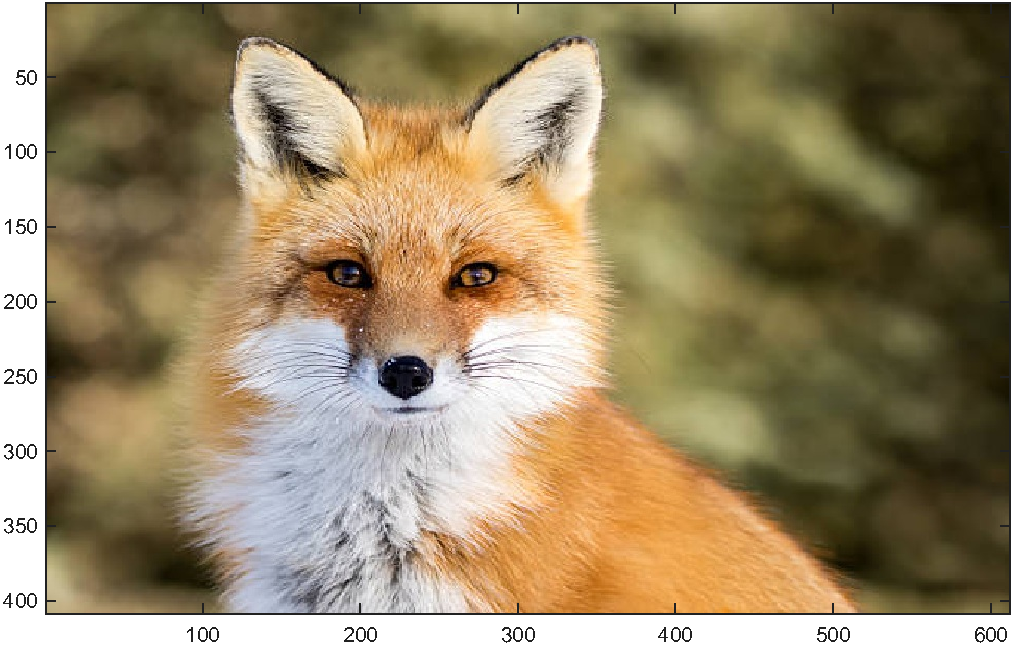
\includegraphics[width=0.8\textwidth]{imagenes/zorro.pdf}
    \caption{Imagen de un zorro cargado en MATLAB}
    \label{fig:1}
\end{figure}


También podemos graficar la misma imagen según el canal de color (figura \ref{fig:2}). 

\begin{lstlisting}[caption = {Procesamiento de imagen en MATLAB}, label = {code:1}]
%# Leo el archivo
l = imread('fox_photo.jpg');
% image(l)

%# Grafico para las primeras 300 columnas
% image(l(:, 1:300, :))

%Grafico para las primeras 300 filas
% image(l(1:300, :, :))

%# canales o colores
R = l(:, :, 1);
G = l(:, :, 2);
B = l(:, :, 3);

% image(B)

%imagen 200x200x3
% image(l(1:200, 1:200, :))

%# Agregamos una linea blanca
figure;
subplot(1, 2, 1);
l(:, 50:75, :) = 255;
image(l)
title('Franja blanca')
axis image;

%# Agregamos una linea negra
subplot(1, 2, 2);
l(150:175, :, :) = 0;
image(l)
title('Franja blanca y negra')
axis image;
\end{lstlisting}


Al igual que podemos graficar la imagen por color, podemos recortarla. Por ejemplo, en la figura \ref{fig:3} recortamos las primeras 200 filas y columnas de la imagen original.


\begin{figure}[ht!]
    \centering
    \begin{subfigure}{0.49\textwidth}
        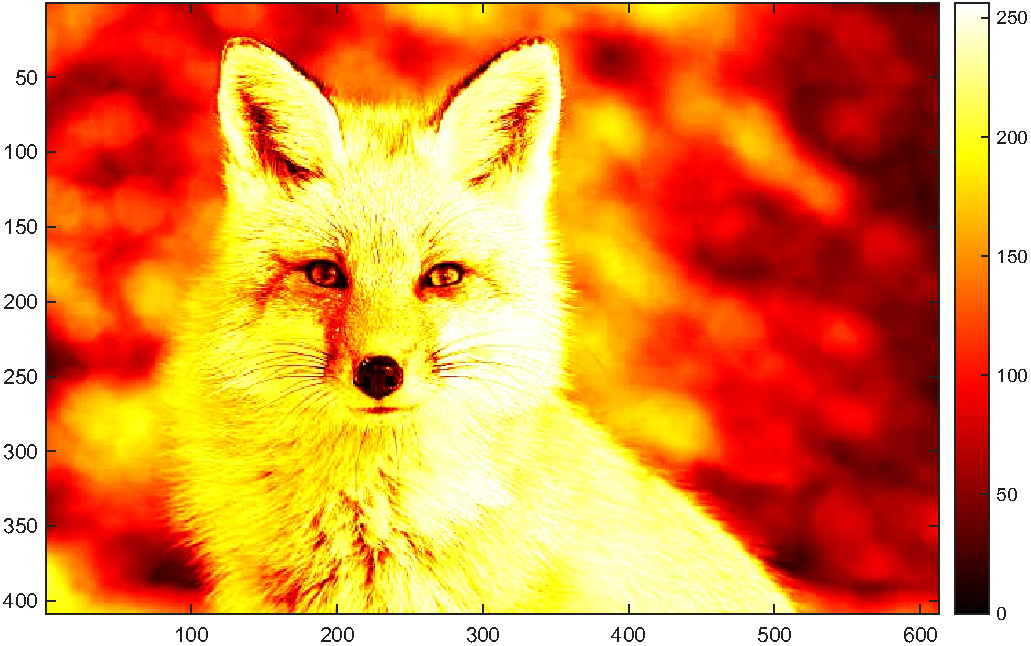
\includegraphics[width=\textwidth]{imagenes/rojo_zorro.pdf}
        \caption{Para el canal rojo: \texttt{image(l(:, :, 1))}}
    \end{subfigure}
    \begin{subfigure}{0.49\textwidth}
        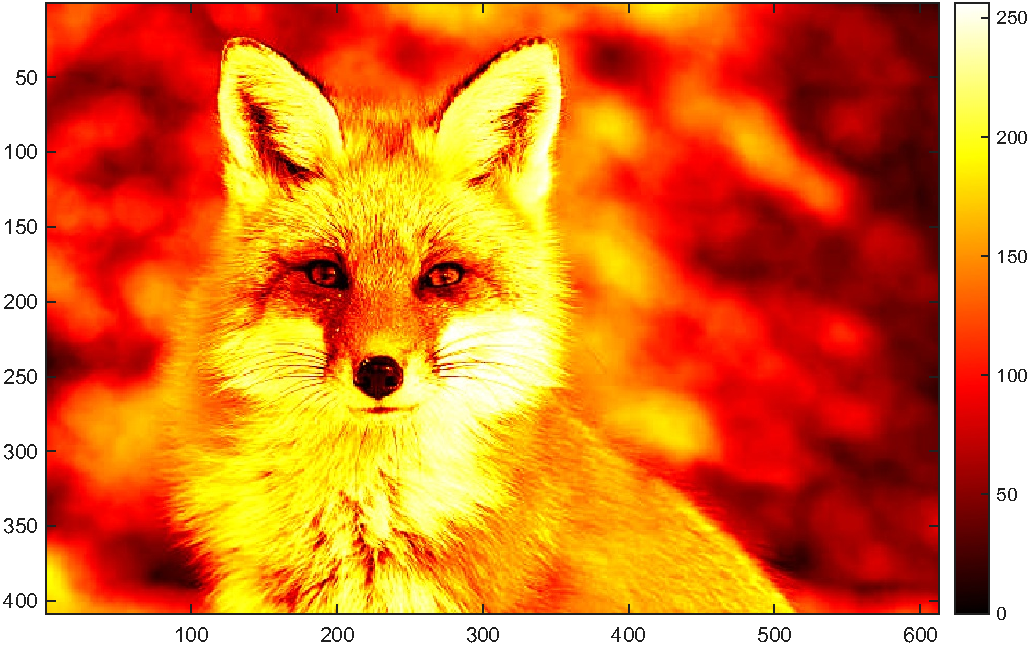
\includegraphics[width=\textwidth]{imagenes/verde_zorro.pdf}
        \caption{Para el canal verde: \texttt{image(l(:, :, 2))}}
    \end{subfigure}
    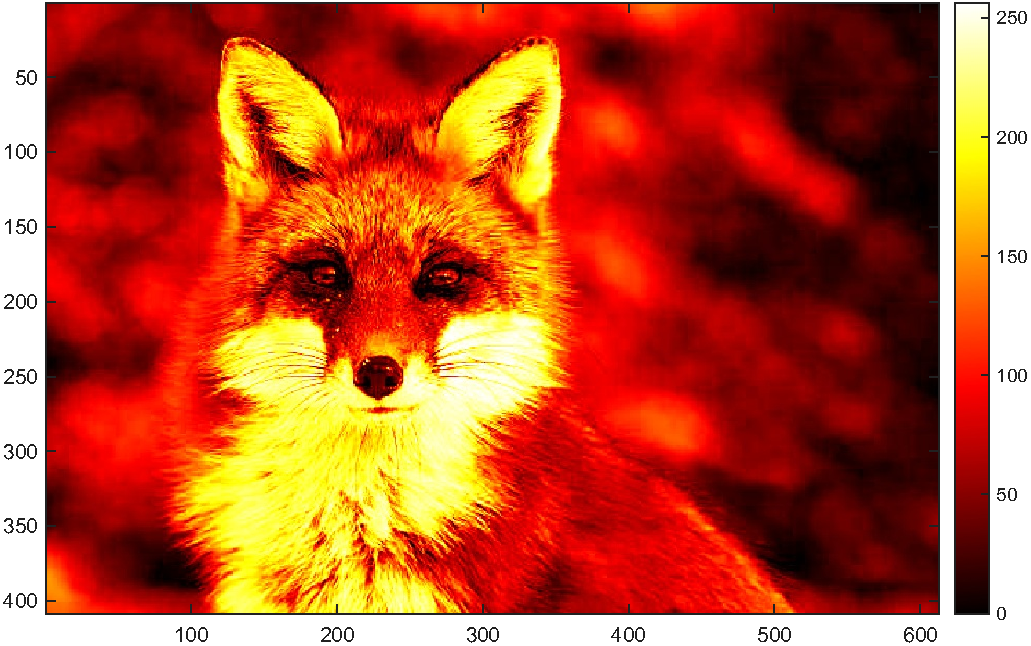
\includegraphics[width = 0.49\textwidth]{imagenes/azul_zorro.pdf}
    \caption{Para el canal azul: \texttt{image(l(:, :, 3))}}
    \label{fig:2}
\end{figure}



\begin{figure}[ht!]
    \centering
    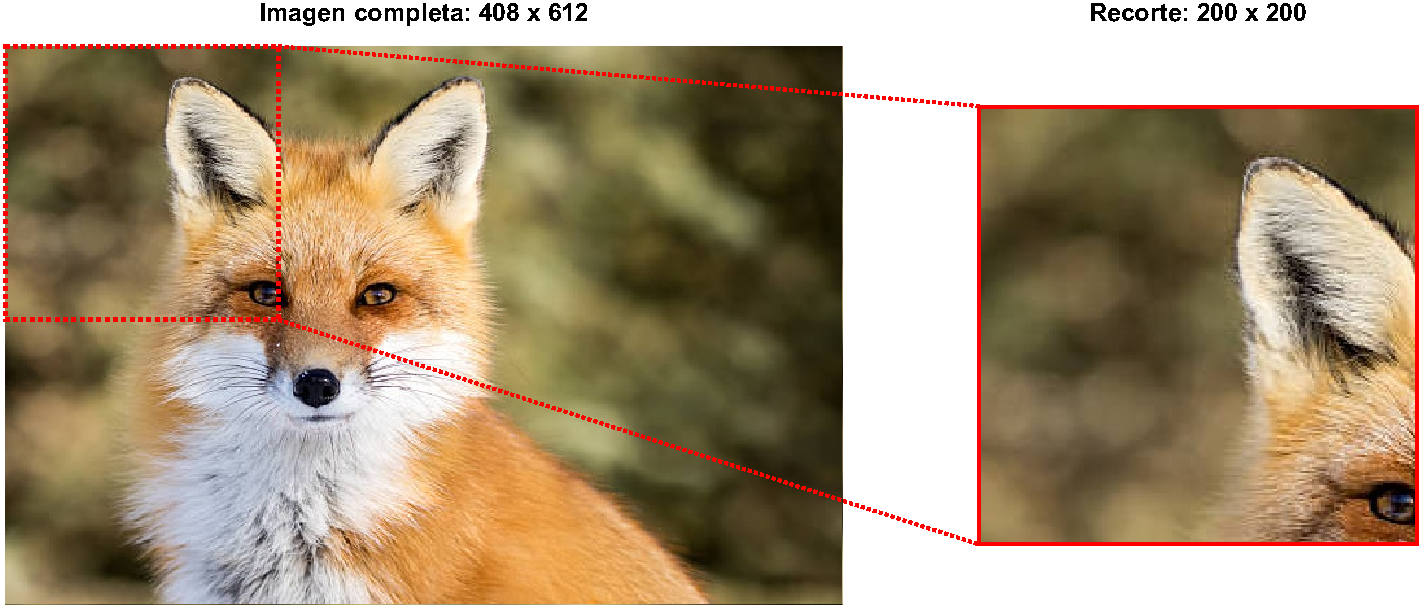
\includegraphics[width=0.8\textwidth]{imagenes/imagen200x200.pdf}
    \caption{Imagen original recortada}
    \label{fig:3}
\end{figure}



Por último, también podemos agregar una línea blanca y negra (ver código \ref{code:1}). En la figura \ref{fig:4} se representan las líneas blancas y negras.

\begin{figure}[ht!]
    \centering
    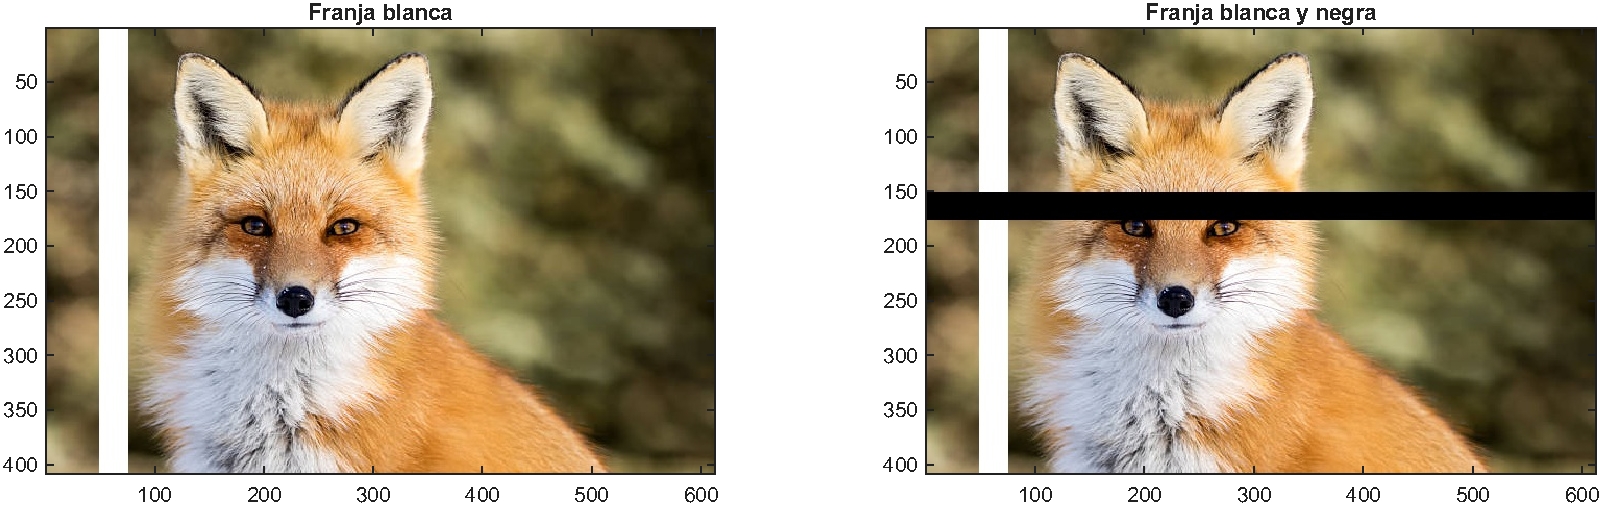
\includegraphics[width=0.9\textwidth]{imagenes/franjas.pdf}
    \caption{Franjas blanca y negra en la imagen original}
    \label{fig:4}
\end{figure}
